%!TEX encoding = UTF-8 Unicode
%!TEX root = ../compendium2.tex

\section{Visual Studio Code med tillägget Scala Metals}\label{appendix:ide:vscode}

Visual Studio Code\footnote{\href{https://en.wikipedia.org/wiki/Visual\_Studio\_Code}{en.wikipedia.org/wiki/Visual\_Studio\_Code}}, förkortat VS Code eller bara \code{code}, är en gratis utvecklingsmiljö som är mestadels öppen källkod\footnote{Varianten VS Codium \url{https://vscodium.com/} är helt fri från stängd källkod.}. Projektet startades och leds av Microsoft och har en aktiv gemenskap med många utvecklare och många användbara tillägg \Eng{extensions}.

VS Code kallas ofta för ''bara'' en editor, men har genom åren utvecklats till en fullfjädrad IDE med bl.a. inbyggd debugger och stöd för många olika språk via ett omfattande bibliotek av tillägg.%

\begin{itemize}
\item 
Läs mer om hur man använder VS Code här: \\
\url{https://code.visualstudio.com/docs}

\item
Läs mer om hur du använder Scala i VS Code här: \\
\url{https://scalameta.org/metals/docs/editors/vscode}

\end{itemize}

Det finns många användbara kortkommandon som gör dig snabbare och snabbare när du kodar, allteftersom du lär dig nya kortkommandon. Ett bra tips är att du lär dig minst ett nytt kortkommando om dagen och efter ett tag kan du riktigt många. Här finns en sammanfattning av de viktigaste kortkommandona för VS Code för Linux:\\
\url{https://code.visualstudio.com/shortcuts/keyboard-shortcuts-linux.pdf}\\
Byt ut \code{linux} mot \code{windows} eller \code{macos} i adressen ovan för motsvarande plattform.

\subsection{Installera VS Code och Metals}\label{appendix:ide:vscode:install}

VS Code är förinstallerad på LTH:s datorer, men du behöver själv installera Scala-tillägget \textbf{Metals} första gången du kör igång VS Code på LTH:s datorer. Läs om installation av Metals här: \\
\url{https://marketplace.visualstudio.com/items?itemName=scalameta.metals} 

Läs mer om hur du installerar VS Code på din egen dator här: \\\url{https://code.visualstudio.com}

Mer information om installation av verktyg finns på kursens hemsida: \\
\url{https://cs.lth.se/pgk/verktyg}

\begin{figure}
\centering
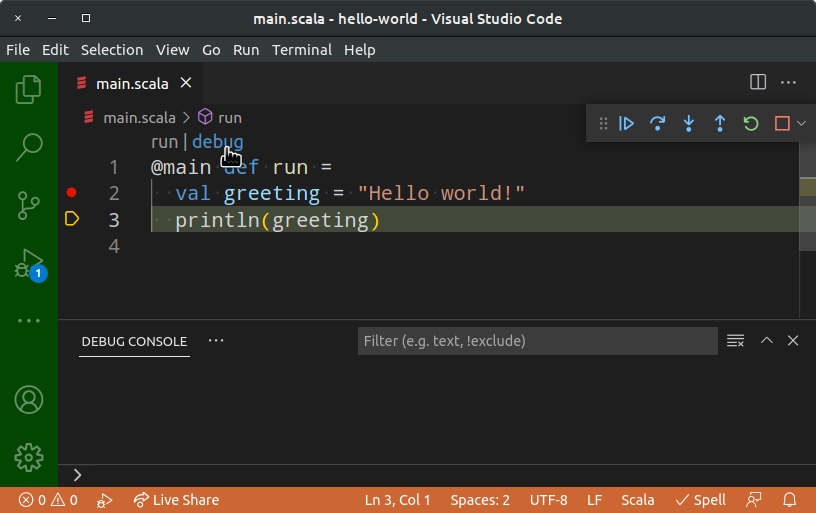
\includegraphics[width=0.9\textwidth]{../img/vscode-debug}
\caption{Debuggern i VS Code.\label{appendix-ide:vscode-debug}}
\end{figure}


\subsection{Använda debuggern i VS Code}

Innan du börjar använda debuggern, läs först om allmän felhantering i Appendix \ref{appendix:debug}.

Du kan aktivera debuggern i VS Code för dina Scala-program genom att klicka på ''debug'' ovanför din \code{main}-metod, förutsatt att du har tillägget Metals installerad i VS Code. Du behöver även köra \texttt{scala-cli setup-ide .} (se Appendix \ref{appendix:compile:scala-cli}), eller ha en giltig \code{build.sbt}-fil (se Appendix \ref{appendix:build}) som du importerar i VS Code när frågan dyker upp i nedre högra hörnet. 

Figur \ref{appendix-ide:vscode-debug} på sidan \pageref{appendix-ide:vscode-debug} visar hur det kan se ut när debuggern i VS Code är aktiverad. Till vänster om radnummerkolumnen kan du klicka för att aktivera och avaktivera brytpunkter. Aktiverade brytpunkter visas som en röd prick i marginalen till vänster. Brytpunkten som är inramad med en gul pil visar den rad som kommer att exekveras härnäst. Notera panelen med olika knappar i överkanten av editorfönstret. Med dessa knappar kan du styra exekveringen enligt följande:
\begin{itemize}
  \item \textbf{Kör vidare}. Den blåa play-knappen kör vidare till nästa brytpunkt, eller tills programmet är klart om inga fler brytpunker påträffas.
  \item \textbf{Stega över}.Den blåa böjda framåtpilen kör en rad i taget \emph{utan} att hoppa in i funktioner.
  \item \textbf{Stega in}. Den blåa nedåtpilen kör vidare en rad i taget och hoppar in i funktioner om raden innehåller funktionsanrop.
  \item \textbf{Stega ut}. Den blåa uppåtpilen kör klar innevarande funktion.
  \item \textbf{Kör igen}. Den gröna återstartsikonen kör om ditt program.
  \item \textbf{Avbryt}. Den röda stoppknappen avbryter denna debuggingsession. Kom ihåg att avbryta innan du startar en ny debuggingsession, annars kan det lätt bli förvirrande med många samtidigt pågående körningar. 
\end{itemize}

Figur \ref{appendix-ide:vscode-trace} på sidan \pageref{appendix-ide:vscode-trace} visar hur VS Code presenterar anropsstacken och värdet på de variabler som syns där exekveringen befinner sig för tillfället. Du får fram detta genom att klicka på ikonen med en lus och en playknapp i det vertikala verktygsfältet längst till vänster.  

\begin{figure}
\centering
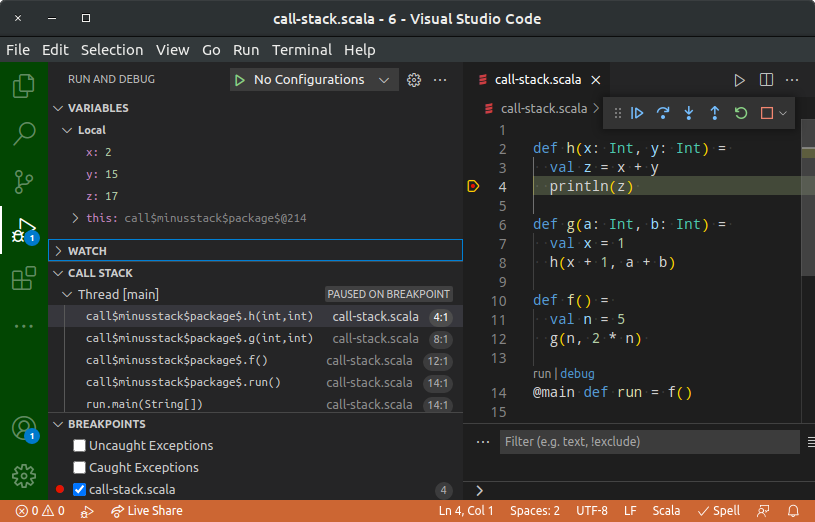
\includegraphics[width=0.9\textwidth]{../img/vscode-trace}
\caption{Anropsstack och variabler i VS Code.\label{appendix-ide:vscode-trace}}
\end{figure}


